% ****************************************************************************************************
\chapter{State of the Art}\label{ch:tf}%Theoretical Foundations
% ****************************************************************************************************

%\begin{flushright}{\slshape    
	%When the wind of change blows,\\
	%some people build walls,\\
	%others build windmills.} \\ \medskip
	%--- Chinese Proverb
%\end{flushright}

In this chapter, the existing research on which this thesis is based is elucidated. First, the term 'business model' and various points of view regarding business models are discussed. Furthermore, one business model conceptualization which is used throughout this thesis is described in detail in Subsection \ref{ch:tf:bmc}. In Section \ref{ch:tf:paas}, the concept of cloud computing, relations to other cloud computing components as well as the \ac{PaaS} domain are introduced. At the end of this chapter, related research on platform strategies as well as modeling and simulating business models is presented.

\section{Business Models}\label{ch:tf:bm}

\begin{flushright}{\slshape    
	There is nothing quite so useless,\\
	as doing with great efficiency, \\
	something that should not be done at all.} \\ \medskip
	--- Peter F. Drucker
\end{flushright}

\vspace*{-18pt}

\subsection{Origins and Definitions}

As early as 1954, Peter F. Drucker proposed the five following questions in order to describe basic business strategies \citep[pp. 49-61]{Drucker1954}:

\begin{enumerate}[parsep=0pt, topsep=0pt, itemsep=0pt]
	\item What is our business?
	\item Who is the customer?
	\item What is value to the customer?
	\item What will our business be?
	\item What should it be?
\end{enumerate}

However, the term 'business model' itself evolved noticeably over time, even continuing in the 90s \mycite{Osterwalder2005}{pp. 3-4}{Zott2011}{p. 1022}. As of the time of writing this paper, there is no generally accepted definition or uniform picture of this concept. According to \citet[p. 726]{Morris2005} and \citet[p. 1022]{Zott2011}, the term 'business model' at a meta level has been referred to as an architecture, an assumption, a conceptual tool or model, a description, a design, a framework, a method, a pattern, a plan, a representation, a set, a statement, as well as a structural template. Therefore, a number of widely used definitions from different points of view are presented below:
	
\begin{quotation}\vspace*{-5pt}{\slshape 
[A business model is] an architecture for the product, service and information flows, including a description of the various business actors and their roles; and a description of the potential benefits for the various business actors; and a description of the sources of revenues.}
\vspace*{-7pt}
\begin{flushright}
	--- \citealp[p. 2]{Timmers1998}
\end{flushright}
\end{quotation}

%\begin{quotation}\vspace*{-5pt}{\slshape 
%Business models are defined as summary of the value creation logic of an organization or a business network including assumptions about its partners, competitors and customers. They define the business and IS architecture, rules, potential benefits and the sources of revenue.}
%\vspace*{-7pt}
%\begin{flushright}
%	--- \citealp[p. 798]{Klueber2000}
%\end{flushright}
%\end{quotation}

\begin{quotation}\vspace*{-5pt}{\slshape 
A business model depicts the content, structure, and governance of transactions designed so as to create value through the exploitation of business opportunities.}
\vspace*{-7pt}
\begin{flushright}
	--- \citealp[p. 511]{Amit2001}
\end{flushright}
\end{quotation}

\begin{quotation}\vspace*{-5pt}{\slshape 
The functions of a business model are to articulate the value proposition, i.e. the value created for users by the offering based on the technology; identify a market segment, i.e. the users to whom the technology is useful and for what purpose, and specify the revenue generation mechanism(s) for the firm; define the structure of the value chain within the firm required to create and distribute the offering, and determine the complementary assets needed to support the firm's position in this chain; estimate the cost structure and profit potential of producing the offering, given the value proposition and value chain structure chosen;  describe the position of the firm within the value network linking suppliers and customers, including identification of potential complementors and competitors; [and] formulate the competitive strategy by which the innovating firm will gain and hold advantage over rivals.}
\vspace*{-7pt}
\begin{flushright}
	--- \citealp[pp. 533-534]{Chesbrough2002}
\end{flushright}
\end{quotation}

%\begin{quotation}\vspace*{-5pt}{\slshape 
%[Business models are] stories that explain how enterprises work. A good business model answers Peter Drucker's age-old questions: Who is the customer? And what does the customer value? It also answers the fundamental questions every manager must ask: How do we make money in this business? What is the underlying economic logic that explains how we can deliver value to customers at an appropriate cost?}
%\vspace*{-7pt}
%\begin{flushright}
%	--- \citealp[p. 2]{Magretta2002}
%\end{flushright}
%\end{quotation}

\begin{quotation}\vspace*{-5pt}{\slshape 
A business model is a concise representation of how an interrelated set of decision variables in the areas of venture strategy, architecture, and economics are addressed to create sustainable competitive advantage in defined markets.}
\vspace*{-7pt}
\begin{flushright}
	--- \citealp[p. 727]{Morris2005}
\end{flushright}
\end{quotation}

%\begin{quotation}\vspace*{-5pt}{\slshape 
%A business model is a conceptual tool that contains a set of elements and their relationships and allows expressing the business %logic of a specific firm. It is a description of the value a company offers to one or several segments of customers and of the architecture of the firm and its network of partners for creating, marketing, and delivering this value and relationship capital, to generate profitable and sustainable revenue streams.}
%\vspace*{-7pt}
%\begin{flushright}
%	--- \citealp[p. 10]{Osterwalder2005}
%\end{flushright}
%\end{quotation}
	
\begin{quotation}\vspace*{-5pt}{\slshape 
[A business model is] a representation of a firm's underlying core logic and strategic choices for creating and capturing value within a value network.}
\vspace*{-7pt}
\begin{flushright}
	--- \citealp[p. 202]{Shafer2005}
\end{flushright}
\end{quotation}

%\begin{quotation}\vspace*{-5pt}{\slshape 
%The particular business concept (or way of doing business) as reflected by the business's core value proposition(s) for customers; its configurated value network to provide that value, consisting of own strategic capabilities as well as other (e.g. outsourced/allianced) value networks; and its continued sustainability to reinvent itself and satisfy the multiple objectives of its various stakeholders.}
%\vspace*{-7pt}
%\begin{flushright}
%	--- \citealp[p. 40]{Voelpel2005}
%\end{flushright}
%\end{quotation}

\begin{quotation}\vspace*{-5pt}{\slshape 
A business model \ldots\xspace consists of four interlocking elements [customer value proposition, profit formula, key resources, and key processes] that, taken together, create and deliver value.}
\vspace*{-7pt}
\begin{flushright}
	--- \citealp[p. 52]{Johnson2008}
\end{flushright}
\end{quotation}

\begin{quotation}\vspace*{-5pt}{\slshape 
A business model describes the rationale of how an organization creates, delivers and captures value.}
\vspace*{-7pt}
\begin{flushright}
	--- \citealp[p. 14]{Osterwalder2010}
\end{flushright}
\end{quotation}

Most of the above-mentioned definitions are focused on the need to filter the complexity of how a company does business through concentrating on its core elements and their interdependencies. \citet[p. 91]{Magretta2002} describes this as follows: \textit{"Business models describe, as a system, how the pieces of a business fit together"}. Furthermore, many business model definitions emphasize the connection with various actors auch as partners, customers, suppliers, and the like, which is also referred to as 'value chain' or 'value network' (\citealp[p. 2]{Timmers1998}; \citealp[pp. 533-534]{Chesbrough2002}; and \citealp[p. 202]{Shafer2005}). Whereas \citet[p. 2]{Timmers1998} explicitly mentions the profitability (for instance benefits) for all members of the value chain, \citet[pp. 533-534]{Chesbrough2002} discuss the need to define the firm's position within the value chain. \citet[p. 727]{Morris2005} and \citet[p. 202]{Shafer2005} highlight that business models depict decision variables and strategic choices and, as such, represent a firm's core logic. In contrast, \citet[p. 2]{Timmers1998} defines business models as an architecture for tangible and intangible asset flows, and \citet[p. 511]{Amit2001} highlight the transactions required to do business. On the other hand, the definitions provided by \citet[p. 52]{Johnson2008} and \citet[p. 14]{Osterwalder2010} describe the big picture of business models, for instance the rationale. \citet[p. 533-534]{Chesbrough2002} provide a comprehensive definition including business model functions like articulation, identification, estimation, description, and formulation.

Further the term business model is often referred to as 'blueprint' \mycite{Osterwalder2005}{p. 2}{Johnson2008}{p. 52}. The blueprint itself constitutes a simplified representation and according to \citet[pp. 11-14]{Osterwalder2005}, enables one to capture, visualize, understand, communicate, and share a company's business logic. Especially for the purpose of communicating and sharing business models, a common framework or language among all stakeholders is essential, so as to avoid misunderstandings of any kind.

The two aspects of value creation and value capture are further terms widely used in the literature on business models. Both concepts are reflected in many business model definitions and conceptualizations, both explicitly and implicitly (\citealp[p. 511]{Amit2001}; \citealp[pp. 533-534]{Chesbrough2002}; \citealp[p. 727]{Morris2005}; \citealp[p. 202]{Shafer2005}; \citealp[p. 12]{Chesbrough2007}; \citealp[p. 52]{Johnson2008}; \citealp[p. 14]{Osterwalder2010}; and \citealp[pp. 1019-1020]{Zott2011}). 

\citet[pp. 729-732]{Morris2005}, in alignment with \citet[pp. 49-61]{Drucker1954}, identify six key questions concerning basic business model components:

\begin{enumerate}[parsep=0pt, topsep=0pt, itemsep=0pt]
	\item How will the firm create value?
	\item For whom will the firm create value?
	\item What is the firm's internal source of advantage?
	\item How will the firm position itself in the marketplace?
	\item How will the firm make money?
	\item What are the entrepreneur's time, scope, and size ambitions?
\end{enumerate}

Even though the concept of business models is moving towards a more mature state, so far few enterprises are able to capture their current business model in a holistic view, including strengths and weaknesses as well as interdependencies \citep[p. 52]{Johnson2008}. This lack of knowledge represents a critical competitive factor, due to the fact that the underlying business model is no less important than the product or technology itself and in some cases even constitutes the basis for success or failure \mycite{Chesbrough2007}{p. 12}{Johnson2008}{p. 52}. According to \citet[p. 50]{Johnson2008}, \textit{"one secret to maintaining a thriving business is recognizing when it needs a fundamental change"}. As an example, these authors describe the need for a fundamental business model adjustment experienced by Hilti, a Liechtenstein-based manufacturer of high-end power tools \citep[pp. 54-57]{Johnson2008}. In the past, Hilti was selling its power tools to contractors, facing more and more intense competition and pressure on margins, for instance from low-end power tools manufacturers. For this reason, Hilti decided to change its business model from scratch in such a way that Hilti is now selling the use of its power tools for a monthly fee instead of the power tools itself.

\subsection{Conceptualization}\label{ch:tf:bmc}

Based on a literature analysis of business model definitions, the definition of \citet{Johnson2008} was taken as a basis for this research. According to \citet[p. 52]{Johnson2008}, \textit{"a business model \ldots\xspace consists of four interlocking elements that, taken together, create and deliver value"}. These four elements are denoted as follows: \ac{CVP}, profit formula, key resources and key processes. In the following, these four elements are described in detail and compared briefly with the Business Model Canvas framework \citep{Osterwalder2010} as well as with other previously mentioned business model definitions. Finally, the reasons why the business model conceptualization of \citet{Johnson2008} is adopted for this thesis are discussed.

The \ac{CVP} is considered as the most crucial part of the business model due to its main objective to satisfy customer needs. In order to understand the customer needs, the following key questions should be answered: 

\begin{enumerate}[parsep=0pt, topsep=0pt, itemsep=0pt]
	\item Who are my target customers?
	\item What is their job to be done (problem)?
	\item How can their problems be solved (offering)? 
\end{enumerate}

The interrelation between the job to be done and the corresponding offer as well as the value of the \ac{CVP} are described by  \citet[p. 52]{Johnson2008} in the following way: \textit{"The more important the job is to the customer, the lower the level of customer satisfaction with current options for getting the job done, and the better your solution is than existing alternatives at getting the job done (and, of course, the lower the price), the greater the \ac{CVP}"}. How a company derives value for itself based on the offering to its customers represents another key element in each business model, termed 'profit formula' here. It consists of the sub-elements revenue model, cost structure, margin model, and resource velocity. Assets which are essential to creating and delivering the above-described \ac{CVP} are summarized as key resources. According to \citet[p. 53]{Johnson2008}, these key resources include people, technology, products, facilities, equipment, channels, as well as the company's brand and reputation. Processes in combination with these assets (key resources) are necessary to deliver the value proposition to the company's customers. These processes need to be efficient, repeatable, and scalable. Key processes include recurring operations such as training, development, manufacturing, budgeting, planning, sales, and services, as well as the company's rules, metrics, and norms \citep[p. 53]{Johnson2008}.

In summary, in the business model conceptualization proposed by \citet[p. 54]{Johnson2008}, the \ac{CVP} represents the value description for the target customers. The value creation and delivery is explained by the two business model elements 'key resources' and 'key processes'. An overview of this business model conceptualization is given in Table \ref{bm:concept}.

Another well-known business model conceptualization or framework is the Business Model Canvas  introduced by \citet{Osterwalder2010}. This framework consists of nine so-called business model 'building blocks', viz. (1) value propositions, (2) customer segments, (3) channels, (4) customer relationships, (5) key activities, (6) key resources, (7) key partners, (8) cost structure, and (9) revenue streams. (For a representation of this conceptual scheme, see Appendix \ref{ch:app02} and Figure \ref{fig:bmc}.) Another conceptualization, consisting of four central dimensions, has been developed by \citet{Frankenberger2013}. The first dimension, "who", answers the following question already proposed by \citet[pp. 49-61]{Drucker1954}, \textit{"Who is the customer?"}. Second, the description of the\linebreak 
\vspace*{-\baselineskip}
% ****************************************************************************************************
% Business Model Concept NEW
% ****************************************************************************************************
\begin{longtable}{L{\column}L{\column}L{\column}L{\column}}
	
	\toprule
	\endfirsthead
	\toprule
	\multicolumn{4}{l}{\textit{continued from previous page (\nameref{bm:concept})}}\\ 
	\midrule
	\endhead
	\midrule
	\multicolumn{4}{r}{\textit{continued on next page}}\\
	\bottomrule
	\endfoot
	\bottomrule
	\caption[Business Model Conceptualization]{Business Model Conceptualization adapted from \citet[p. 54]{Johnson2008}}
	\label{bm:concept}
	\endlastfoot
	
	\multicolumn{4}{c}{\textbf{Customer Value Proposition (CVP)}}\\ \midrule
	
	\textbf{\small Target customer} &
	\small \textbf{Job to be done} to solve an important problem or fulfill an important need for the target customer. &
	\multicolumn{2}{L{\columnT}}{\small \textbf{Offering}, which satisfies the problem or fulfills the need. This is defined not only by what is sold but also by how it's sold.} \\ 

% KEY RESOURCES
\multicolumn{2}{L{\columnT}}{\textbf{Key Resources} \small needed to deliver the customer value proposition profitably. Might include:
\begin{itemize}[leftmargin=*, parsep=0pt, topsep=0pt, itemsep=0pt]
	\item \textbf{People}
	\item \textbf{Technology, products}
	\item \textbf{Equipment}
	\item \textbf{Information}
	\item \textbf{Channels}
	\item \textbf{Partnerships, alliances}
	\item \textbf{Brand}\vspace{-\baselineskip} 
\end{itemize}
} &
\multicolumn{2}{L{\columnT}}{\textbf{Key Processes} \small as well as rules, metrics, and norms, that make the profitable delivery of the customer value proposition repeatable and scalable. Might include:
\begin{itemize}[leftmargin=*, parsep=0pt, topsep=0pt, itemsep=0pt]
	\item \textbf{Processes:} design, product development, sourcing, manufacturing, marketing, hiring and training, IT
	\item \textbf{Rules and metrics:} margin requirements for investment, credit terms, lead times, supplier terms
	\item \textbf{Norms:} opportunity size needed for investment, approach to customers and channels\vspace{-\baselineskip} 
\end{itemize}} \\ \midrule

% PROFIT FORMULA
\multicolumn{4}{L{\columnF}}{\textbf{Profit Formula} \small
\begin{itemize}[leftmargin=*, parsep=0pt, topsep=0pt, itemsep=0pt]
		\item \textbf{Revenue model:} How much money can be made: price x volume. Volume can be thought of in terms of market size, purchase frequency, ancillary sales, etc.
		\item \textbf{Cost structure:} How costs are allocated: includes cost of key assets, direct costs, indirect costs, economies of scale.
		\item \textbf{Margin model:} How much each transaction should net to achieve desired profit levels. 
		\item \textbf{Resource velocity:} How quickly resources need to be used to support target volume. Includes lead times, throughput, inventory turns, asset utilization, and so on.\vspace{-\baselineskip} 
\end{itemize} 
}\\ 
\end{longtable}



 
\noindent value proposition for the customer represents the next dimension, "what". This dimension, too, was already mentioned by \citet[pp. 49-61]{Drucker1954}: \textit{"What is value to the customer?"}. The third dimension describes the value creation and delivery, the "how", and answers the following question proposed by \citet[pp. 729-732]{Morris2005}, \textit{"How will the firm create value?"}. And finally, the profitability of a business model is described through the fourth dimension, "why", which answers the question mentioned by \citet[pp. 729-732]{Morris2005}, \textit{"How will the firm make money?"}. These four dimensions can be found in almost all business model definitions.

In simplified terms, the bottom part of the Business Model Canvas -- cost structure and revenue streams -- deals with the value capture aspect or, in other words, why a company should perform (or is performing) the described business model. The seven remaining building blocks, i.e. value propositions, customer segments, channels, customer relationships, key activities, key resources, and key partners, represent the value creation aspect. In other words, the upper left-hand side answers the how, the center part (value propositions) the what, and the right-hand side the who-question. Also, the six basic questions concerning business models from \citet[pp. 729-732]{Morris2005} mentioned above correspond to the four dimensions proposed by \citet{Frankenberger2013}. Only the sixth question -- \textit{"What are the entrepreneur's time, scope, and size ambitions?"} -- cannot be easily assimilated to the business model conceptualizations from \citet{Johnson2008}, \citet{Osterwalder2010}, and \citet{Frankenberger2013}, due to fact that this question is concerned with strategic issues, for instance growth or speculative models. Although the above-mentioned business model conceptualizations (and also the previously introduced business model definitions) differ in the total number of business model elements or questions they include, they are largely equivalent. In Table \ref{tab:bmcc}, the business model elements according to \citet{Johnson2008}, \citet{Osterwalder2010}, \citet{Morris2005}, and \citet{Frankenberger2013} are compared and contrasted.

\begin{table}[t]
	\caption{Comparison of Business Model Conceptualizations}
	\label{tab:bmcc}
	\centering
	\begin{tabular}{L{.2\textwidth}L{.2\textwidth}L{.2\textwidth}L{.2\textwidth}}
			\toprule 
			\footnotesize \textbf{\citet{Johnson2008}} & \footnotesize \textbf{\citet{Osterwalder2010}} & \footnotesize \textbf{\citet{Morris2005}} & \footnotesize \textbf{\citet{Frankenberger2013}} \\ \midrule
			\footnotesize Customer Value Proposition & \footnotesize Customer Segments \newline Value Propositions & \footnotesize For whom will the firm create value? \newline How will the firm create value? & \footnotesize Who \newline ~ \newline What \\ \midrule
			\footnotesize Profit Formula	& \footnotesize Cost Structure\newline Revenue Streams & \footnotesize How will the firm make money? & \footnotesize Why\\ \midrule
			\footnotesize Key Resources & \footnotesize Key Resources\newline Key Partners\newline Channels & \footnotesize What is the firm's internal source of advantage?& \footnotesize How\\ \midrule
			\footnotesize Key Processes & \footnotesize Key Activities \newline Customer Relationships & \footnotesize How will the firm position itself in the marketplace? & \footnotesize How\\ \bottomrule
	\end{tabular}
\end{table}

Platform-based business models are by nature two-sided or even multi-sided with respect to the customer segments and the corresponding value propositions. Whereas the Business Model Canvas is particularly appropriate for one-sided business models, there is a major shortcoming restricting its utilization in the domain of platform-based business models. In terms of \citet{Johnson2008}, each customer segment has its own problem (job to de done) and needs a corresponding offering (value proposition). Thus, it is crucial to differentiate between different customer segments in platform-based business models. The Business Model Canvas framework cannot easily be extended (the upper center and right-hand side of this conceptual scheme, especially the two elements 'value proposition' and 'customer segments') to take into account several disjoint customer segments and their corresponding value propositions. The framework proposed by \citet{Johnson2008}, however, can easily accommodate more than one customer segment, due to the fact that several \acp{CVP}, including the customer segment (target customer) and their value proposition (offering), are possible. Hence, the business model conceptualization by \citet{Johnson2008} is used as a reference framework in this thesis.

\section{Cloud Computing}\label{ch:tf:paas}
\begin{flushright}{\slshape 
	In pioneer days they used oxen for heavy pulling,\\
	and when one ox couldn't budge a log,\\
	they didn't try to grow a larger ox.\\
	We shouldn't be trying for bigger computers,\\
	but for more systems of computers.} \\ \medskip
	--- Grace Hopper
\end{flushright}

\vspace*{-18pt}

\subsection{Origins and Definitions}

In the recent past, a new computing paradigm in the \ac{IT} industry has emerged -- cloud computing, which is also referred to as utility computing. Due to the fact that cloud computing is still relatively new, no generally accepted definition, or even standardization, has so far been developed, although a considerable amount of theoretical and applied research has been published. Despite its general and broad character the following definition provided by the \ac{NIST} is well-established and widely used:

\begin{quotation}{\slshape 
Cloud computing is a model for enabling ubiquitous, convenient, on-demand network access to a shared pool of configurable computing resources (e.g., networks, servers, storage, applications, and services) that can be rapidly provisioned and released with minimal management effort or service provider interaction.}
\vspace*{-7pt}
\begin{flushright}
	--- \citealp[p. 2]{Mell2011}
\end{flushright}
\end{quotation}

Based on a comprehensive literature review of current cloud computing definitions, \citet{Vaquero2009} identify ten essential cloud characteristics -- user friendliness, virtualization, internet centric, variety of resources, automatic adaptation, scalability, resource optimization, pay per use, infrastructure \acp{SLA}, and service \acp{SLA}. Not all of these characteristics are used throughout all the investigated definitions. However, a few of them are widely accepted and led \citet{Vaquero2009} to derive a minimal cloud computing definition, encompassing \textit{"scalability, pay-per-use utility model and virtualization"} \citep[p. 51]{Vaquero2009}. Besides this minimal definition, a more comprehensive consensus definition has been extracted:

\begin{quotation}{\slshape 
Clouds are a large pool of easily usable and accessible virtualized resources (such as hardware, development platforms and/or services). These resources can be dynamically reconfigured to adjust to a variable load (scale), allowing also for an optimum resource utilization. This pool of resources is typically exploited by a pay-per-use model in which guarantees are offered by the Infrastructure Provider by means of customized \acp{SLA}.}
\vspace*{-7pt}
\begin{flushright}
	--- \citealp[p. 51]{Vaquero2009}
\end{flushright}
\end{quotation}

There are three layers inherent in the concept of cloud computing (\citealp[pp. 118-119]{Iyer2010} and \citealp[pp. 2-3]{Mell2011}), also referred to as cloud stack (cf. Figure \ref{fig:ccs}). The \ac{SaaS} layer is the most visible layer of cloud computing for end users, since it is here that they access the on-demand applications the software vendor provides, without the need to manage or control the underlying infrastructure. Next, the \ac{PaaS} layer enables to develop and deploy applications as well as services onto cloud infrastructure (a detailed introduction is provided in Subsection \ref{ch:tf:paas:def}). Finally, the \ac{IaaS} layer encompasses the provision of various computing resources, for instance processing, storage, and network capabilities. In contrast to \citet[p. 50]{Armbrust2010}, in this thesis the \ac{IaaS} and \ac{PaaS} layer are considered as two different concepts, and not as similar or indiscernible ones. 

\begin{figure}[tb]
	\centering
	% ****************************************************************************************************
% Classification Procedural Model
% ****************************************************************************************************

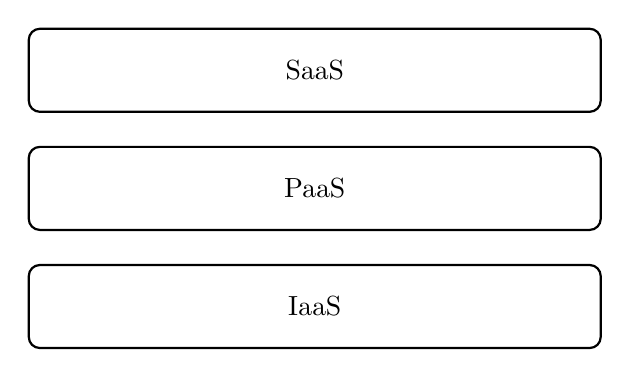
\begin{tikzpicture}%[scale=0.75, every node/.style={scale=0.75}]

\node[draw,text width=20em,text centered,rectangle,rounded corners,minimum height=3em,thick] (1) at (0,3) {\acf{SaaS}};
\node[draw,text width=20em,text centered,rectangle,rounded corners,minimum height=3em,thick] (2) at (0,1.5) {\acf{PaaS}};
\node[draw,text width=20em,text centered,rectangle,rounded corners,minimum height=3em,thick] (3) at (0,0) {\acf{IaaS}};

\end{tikzpicture}
	\caption{Cloud Computing Stack}
	\label{fig:ccs}
\end{figure}

According to \citet[p. 3]{Mell2011}, four deployment models are commonly used. First, private clouds are designed for a single specific entity and are managed by the entity itself or a third party. Second, several entities jointly operate a community cloud to support a shared goal or mission. Third, public clouds are owned by an organization and open to the general public or a designated domain. And fourth, any combination of two or more of the above-mentioned clouds is denoted a hybrid cloud.
Several authors have identified a number of features of cloud computing, which are listed below to provide a broad overview. \citet[pp. 54-58]{Armbrust2010} identify ten obstacles for cloud computing -- three concerning the adoption (availability/business continuity, data lock-in, data confidentiality and auditability), the next five affecting the growth (data transfer bottlenecks, performance unpredictability, scalable storage, bugs in large distributed systems, and scaling quickly), and the last two are business obstacles (reputation fate sharing and software licensing). \citet[pp. 120-127]{Iyer2010} describe seven cloud computing capabilities -- controlled interface, location independence, sourcing independence, ubiquitous access, virtual business environments, addressability and traceability, and rapid elasticity. And finally, \citet[p. 2]{Mell2011} highlight five essential characteristics in this field -- on-demand self-service, broad network access, resource pooling, rapid elasticity, and measured service. 

\citet{Smith2012} analyzes the cloud computing environment and reasons that cloud computing with its various sub-concepts, like \ac{IaaS}, \ac{PaaS}, and \ac{SaaS}, is still an evolving area. However, the individual sub-concepts are currently at different stages of development. According to \citet[p. 5]{Smith2012}, the \ac{IaaS} and especially the \ac{SaaS} layer are already quite advanced and will reach the so-called \textit{"Plateau of Productivity"} in the near future, whereas the \ac{PaaS} layer is currently at a stage labeled \textit{"Peak of Inflated Expectations"} \citep[p. 5]{Smith2012}, and further research is necessary to determine the actual capabilities of this layer. The complete picture of this study can be found in Appendix \ref{ch:app03} (cf. Figure \ref{fig:cloudCycle}). \citet[p. 120]{Iyer2010} also point out that the cloud computing area is still evolving, the \ac{IaaS} layer being the prevalent sub-concept.

Cloud computing and its features are appealing for \acp{SME}, due to their limited \ac{IT} in-house resources and knowledge in combination with growing \ac{IT} requirements and needs (\citealp[p. 398]{Weinhardt2009} and \citealp{Karabek2011}). Benefits inherent in cloud computing, regardless of the customer size, are increased flexibility, reliability, as well as agility to respond to internal and external demands (\citealp[p. 51]{Vaquero2009} and \citealp[p. 129]{Iyer2010}). Moreover, a company's first forays into cloud computing are not accompanied by high entry or upfront investment costs and the use of cloud computing enables companies to convert capital expenses to operating expenses, or, in other words, to convert fixed costs into variable costs, hence gaining the possibility of focusing on their core business \citep[pp. 51-53]{Armbrust2010}. In their current state, most cloud computing offers are not priced based on classical license agreements, but rather based on usage, which is labeled as pay-as-you-go or pay-per-use pricing (\citealp[pp. 50-54]{Vaquero2009}; \citealp[pp. 51-53,58]{Armbrust2010}; and \citealp[p. 2]{Iyer2010}). A comprehensive overview of software pricing strategies is provided by \nolinebreak\citet{Lehmann2009}.

\begin{figure}[t]
	\centering
	\begin{subfigure}{.75\textwidth}
		\centering
		% ****************************************************************************************************
% Capacity Cloud
% ****************************************************************************************************

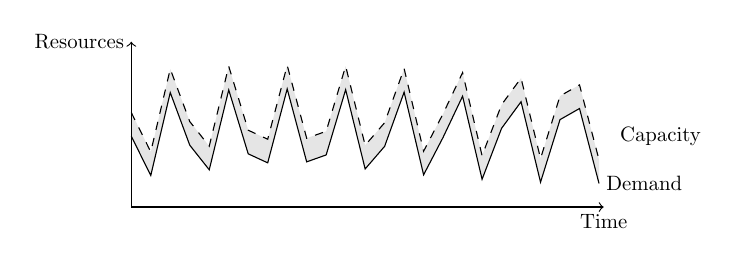
\begin{tikzpicture}[scale=0.6, every node/.style={scale=0.75}]

\fill[fill=gray!20] (0,1.5) -- plot [domain=0:9.9](\x, {sin(10*(\x r)) + 1.5}) -- plot[domain=9.9:0] (\x, {sin(10*(\x r)) + 2}) (0,1.5);

\draw[<->]  (10,0) node[below]{Time} -- (0,0) -- (0,3.5) node[left]{Resources};
\draw [domain=0:9.9] plot (\x, {sin(10*(\x r)) + 1.5})node[right]{Demand};
\draw [domain=0:9.9,dashed] plot (\x, {sin(10*(\x r)) + 2});
\node(1) at (11.2,1.5){Capacity};


\end{tikzpicture}



		\caption{On-Demand}\label{fig:rpc}
	\end{subfigure}
	\begin{subfigure}[b]{.75\textwidth}
		\centering
		% ****************************************************************************************************
% Capacity Static - Underprovisioning
% ****************************************************************************************************

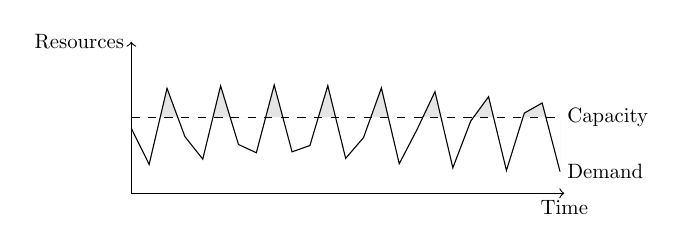
\begin{tikzpicture}[scale=0.55, every node/.style={scale=0.75}]

\fill[fill=gray!20] (0,1.75) -- plot [domain=0:9.9](\x, {sin(10*(\x r)) + 1.5}) -- (9.9,1.75) -- (0,1.75);
\fill[fill=white] (0,1.75) -- (9.9,1.75) -- (9.9,0) -- (0,0) -- (0,1.75);

\draw[<->]  (10,0) node[below]{Time} -- (0,0) -- (0,3.5) node[left]{Resources};
\draw [domain=0:9.9,dashed] (0,1.75) -- (9.9,1.75)node[right]{Capacity};
\draw [domain=0:9.9] plot (\x, {sin(10*(\x r)) + 1.5})node[right]{Demand};

\end{tikzpicture}



		\caption{Underprovisioning}\label{fig:rpu}
	\end{subfigure}
	\begin{subfigure}[b]{.75\textwidth}
		\centering
		\input{gfx/capacityStaticOver}
		\caption{Overprovisioning}\label{fig:rpo}
	\end{subfigure}
	\caption[Resource Provisioning]{Resource Provisioning, adapted from \citet[p. 54]{Armbrust2010} and \citet[p. 127]{Iyer2010}}
	\label{fig:rp}
\end{figure}

One of the key features of cloud computing and its sub-concepts is the ability to scale according to the required demand, also referred to as elasticity (\citealp[p. 4]{Foster2008}; \citealp[pp. 52-54]{Armbrust2010}; \citealp[p. 126]{Iyer2010}; \citealp[pp. 9-10]{Zhang2010}; and \citealp[p. 2]{Mell2011}). In order to provide a flexible utilization of resources, cloud providers use the concepts of virtualization and statistical multiplexing. By using these functionalities, a cloud service can scale up nearly in real-time, thereby allocating enough resources to cope with dynamic workloads (cf. Figure \ref{fig:rpc}). In contrast to cloud services, static on-premise systems cannot easily scale dynamically and by no means in real-time. For this kind of system, a managerial decision about the expected peak load is required to determine the computing capacity necessary to manage this load. Two scenarios, both of which less than optimal, typically arise in this kind of situation. First, the peak load is underestimated and consequently the available computing capacity is incapable of handling the actual peak loads (cf. Figure \ref{fig:rpu}). And second, the peak load is overestimated and hence a large part of the computing resources remains permanently idle, in other words, the available resources are underutilized (cf. Figure \ref{fig:rpo}). Undoubtedly, these two cases represent risks for companies -- either systems with high response times or a waste of money. The utilization of cloud services enables companies to shift these risks largely to the cloud providers and thus to retain the ability to act flexibly.

\subsection{Platform as a Service}\label{ch:tf:paas:def}

In the following, a few more definitions are provided for a better understanding of platforms and in particular the \ac{PaaS} layer. These insights will be helpful in the remainder of this thesis. Product platforms are defined generally by \citet{Halman2003} as follows:

\begin{quotation}{\slshape 
A platform \ldots\xspace is neither the same as an individual product, nor is it the same as a product family; it is the common basis of all individual products within a product family. \ldots\xspace The leading principle behind the platform concept is to balance the commonality potential and differentiation needs within a product family. \ldots\xspace [Therefore, product platforms are considered] as a set of subsystems and interfaces that form a common structure from which a stream of related products can be developed and produced efficiently.}
\vspace*{-7pt}
\begin{flushright}
	--- \citealp[pp. 150-151]{Halman2003}
\end{flushright}
\end{quotation}

Within the \ac{IT} industry many (technical) platforms are prevalent -- for instance operating systems (i.e. Microsoft Windows, OS X, GNU/Linux, and UNIX) and web browsers (i.e. the Mozilla Firefox web browser with its diverse add-ons). \citet{Poel2007} define platforms within the \ac{IT} industry in the following way:

\begin{quotation}{\slshape 
[Platforms] refer to a hardware configuration, an operating system, a software framework or any other common entity on which a number of associated components or services run.}
\vspace*{-7pt}
\begin{flushright}
	--- \citealp[p. 88]{Poel2007}
\end{flushright}
\end{quotation}

Similarly, but more focused on software platforms, \citet{Tiwana2010} define the core concepts of these platforms as follows:

\begin{quotation}{\slshape 
[A software platform is] the extensible codebase of a software-based system that provides core functionality shared by the modules that interoperate with it and the interfaces through which they interoperate. [A module is] an add-on software subsystem that connects to the platform to add functionality to the platform. The collection of the platform and the modules specific to it [is labeled an ecosystem]. [Interfaces are] specifications and design rules that describe how the platform and modules interact and exchange information.}
\vspace*{-7pt}
\begin{flushright}
	--- \citealp[p. 676]{Tiwana2010}
\end{flushright}
\end{quotation}

Based on these introductory platform definitions, more extensive characterizations of platforms in the area of cloud computing, also known as the \ac{PaaS} layer, will now be presented. The first quote describes the actual functioning of the \ac{PaaS} layer whereas the second one defines the purpose of the\ac{PaaS} layer in general:

\begin{quotation}{\slshape 
The capability provided to the consumer is to deploy onto the cloud infrastructure consumer-created or acquired applications created using programming languages, libraries, services, and tools supported by the provider. [Footnote in the original source: This capability does not necessarily preclude the use of compatible programming languages, libraries, services, and tools from other sources.] The consumer does not manage or control the underlying cloud infrastructure including network, servers, operating systems, or storage, but has control over the deployed applications and possibly configuration settings for the application-hosting environment.}
\vspace*{-7pt}
\begin{flushright}
	--- \citealp[pp. 2-3]{Mell2011}
\end{flushright}
\end{quotation}

\begin{quotation}{\slshape
[The \ac{PaaS} layer] facilitates the development and deployment of applications without the cost and complexity of buying and managing the underlying hardware and software layers.}
\vspace*{-7pt}
\begin{flushright}
	--- \citealp[p. 178]{Marston2011}
\end{flushright}
\end{quotation}

These five quotes should help to elucidate both, the concept of a platform in general as well as the way it applies to the area of cloud computing. To sum up, \citet[pp. 150-151]{Halman2003} define platforms in general and clarify that a platform constitutes the common basis for several products, while still enabling these products to differentiate themselves essentially from each other. \citet[p. 88]{Poel2007} define platforms within the \ac{IT} industry in a broad manner. In more detail and with special regard to software platforms, \citet[p. 676]{Tiwana2010} define these platforms as consisting of the core platform (i.e. the extensible codebase), the modules (i.e. platform add-ons), as well as an interface (i.e. the linkage between the platform and the modules). All elements together are denoted an ecosystem. A similar point of view can also be found in the definition provided by \citet[pp. 150-151]{Halman2003}. In order to use a common language and understanding of platforms, the terminology introduced by \citet{Tiwana2010} is used throughout this thesis, i.e. platform, module, interface, and ecosystem.  	

\citet[pp. 2-3]{Mell2011} describe the \ac{PaaS} layer as the capability to deploy acquired or self-developed applications, which are under the user's control, onto cloud infrastructure which is not managed or controlled by the \ac{PaaS} user. In a similar way but with a larger scope, \citet[p. 178]{Marston2011} define the \ac{PaaS} layer as encompassing the development and deployment of applications without the need to manage the underlying layers. Due to its broad character, the \ac{PaaS} definition of \citet[p. 178]{Marston2011} is used in this paper. 

In simplified terms, the \ac{PaaS} layer abstracts the \ac{IaaS} layer (including the automated resource management) and provides a runtime environment in which applications and services run. Usually, these software platforms are open to external developers and offer a kind of development environment, either online (i.e. browser-based) or offline (i.e. \ac{SDK}). Sometimes both variants are provided. Furthermore, these development environments address different stakeholders, ranging from technical developers to business people, and thus vary from comprehensive \acp{IDE} to graphical drag and drop environments. A powerful dashboard, including features to administrate and manage applications as well as service-related issues, commonly completes the \ac{PaaS} offer. As mentioned earlier, according to \citet[p. 5]{Smith2012}, the \ac{PaaS} layer is currently located at the so-called \textit{"Peak of Inflated Expectations"} (cf. Appendix \ref{ch:app03}) and consequently some of the current \ac{PaaS} providers will be driven out of the market and new \ac{PaaS} providers will emerge. Furthermore, it is to be expected that competition between \ac{PaaS} providers will increase constantly. \citet[pp. 117,128-129]{Iyer2010} describe those rivalries as ecosystem-based or network-based competiton. In the same vein, \citet[pp. 675-676]{Tiwana2010} notice a shift of competition towards platform-centric ecosystems.

\section{Related Research}\label{ch:tf:rw}

In this section, relevant research from the large areas of platform strategies as well as modeling and simulating business models is presented.

\subsection{Platform Strategies}\label{ch:tf:rw:ps}

\citet{Cusumano2010} investigates how platforms and the platform adoption can be a decisive factor in the success of different products and technologies. Especially in the \ac{IT} industry, companies with industry-wide platforms are dominant and most successful. An industry platform is loosely defined as a core technology whose comparably low inherent value is enhanced by external components provided by third party companies, named as complementators. As typical examples, the Windows-Intel personal computers as well as smart phones are mentioned. In order to attract the complementators and become an industry-wide platform, companies need a strong strategy for opening their core technology as well as for creating platform incentives. Standards themselves are often wrongly considered to be platforms. Nevertheless, standards can be an important part of the strategy. The critical feature of industry-wide platforms are, both direct and indirect, network effects, which create positive feedback loops and can enable and support high platform adoption rates. As an inherent feature of \ac{PaaS} business models, \citet{Cusumano2010} points out that platform industries often tend to address more than one market side and names such platforms multi-sided platforms, for instance addressing end users, application developers, advertisers, and producers of content in the area of social networking. An adequate strategy is difficult to design and needs to take all essential matters into account. The paper concludes with the groundbreaking ending, \textit{"who wins and who loses these competitions is not simply a matter of who has the best technology or the first product. It is often who has the best platform strategy and the best ecosystem to back it up"} \citep[p. 34]{Cusumano2010}.

The questions which platform strategies are predestinated to become platform leaders as well as how to establish a vibrant ecosystem were investigated by \citet{Gawer2008}. Companies of all sizes can become platform leaders under the right circumstances, although for financially successful companies some aspects are comparably easier to achieve. However, oftentimes companies which are trying to establish an industry platform based on their product(s), called platform-leader wannabes, experience failure. Certainly not all products can become an industry-wide platform. According to \citet[p. 29]{Gawer2008}, a product has the potential to become a platform just in case the following two prerequisites are satisfied: \textit{"(1) It should perform at least one essential function within what can be described as a 'system of use' or solve an essential technological problem within an industry, and (2) it should be easy to connect to or to build upon to expand the system of use as well as to allow new and even unintended end-uses"}. These two conditions are not at all sufficient to become an industry platform, nevertheless they constitute an initial indicator of the potential platform eligibility. As a general rule, platform-leader wannabes already need to take into account business and technology aspects of platform leadership at an early stage of development. Platform-leader wannabes find themselves either in the situation of creating a new platform for an as of yet unsolved problem or in the situation of a platform war with other platform-leader wannabes. For both situations different technology and business actions have been identified, which are presented in Table \ref{tab:plw}. Based on an empirical analysis, \citet{Gawer2008} conclude that identifying platform-like technologies is more simply compared to finding the corresponding business strategy.

\begin{table}[t]
	\caption[Strategic Options for Platform-Leader Wannabes]{Strategic Options for Platform-Leader Wannabes, adapted from \citet[p. 32]{Gawer2008}}
	\label{tab:plw}
	\centering
	\begin{tabular}{L{.45\textwidth}L{.45\textwidth}}
			\toprule 
			\footnotesize \textbf{Coring: How to Create a New Platform Where None Existed Before} & 
			\footnotesize \textbf{Tipping: How to Win Platform Wars By Building Market Momentum} \\ \midrule
			\multicolumn{2}{c}{\footnotesize Technology Actions to Consider:} \\
			\vspace{-4mm}
			\footnotesize
			\begin{itemize}[leftmargin=*, parsep=0pt, topsep=0pt, itemsep=0pt]
				\item  Solve an essential "system" problem
				\item Facilitate external companies' provision of add-ons
				\item Keep intellectual property closed on the innards of your technology
				\item Maintain strong interdependencies between platform and complements\vspace{-\baselineskip} 
			\end{itemize} &
			\vspace{-4mm}
			\footnotesize
			\begin{itemize}[leftmargin=*, parsep=0pt, topsep=0pt, itemsep=0pt]
				\item Try to develop unique, compelling features that are hard to imitate and that attract users
				\item Tip across markets: absorb and bundle technical features from an adjacent market \vspace{-\baselineskip} 
			\end{itemize}\\ \midrule
			\multicolumn{2}{c}{\footnotesize Business Actions to Consider:} \\
			\vspace{-4mm}
			\footnotesize
			\begin{itemize}[leftmargin=*, parsep=0pt, topsep=0pt, itemsep=0pt]
				\item Solve an essential business problem for many industry players
				\item Create and preserve complementors' incentives to contribute and innovate
				\item Protect your main source of revenue and profit
				\item Maintain high switching costs to competing platforms	\vspace{-\baselineskip} 
			\end{itemize} &
			\vspace{-4mm}
			\footnotesize
			\begin{itemize}[leftmargin=*, parsep=0pt, topsep=0pt, itemsep=0pt]
				\item Provide more incentives for complementors than your competitors do
				\item Rally competitors to form a coalition
				\item Consider pricing or subsidy mechanisms that attract users to the platform \vspace{-\baselineskip} 
			\end{itemize} \\ \bottomrule
	\end{tabular}
\end{table}

In addition to approaches enabling platform leadership, \citet{Cusumano2002} identify several elements of platform leadership. In total four disjunct yet tightly related levers of platform leadership have been identified, viz. (1) scope, (2) product technology, (3) relationships with external complementors, and (4) internal organization. These levers can support representatives in the process of formulating the platform strategy with respect to both business and technology characteristics. In the following the four levers are briefly described. First, the scope defines how and where complements are mainly developed -- in-house or by complementors. In the former case, the platform leader needs to establish the required capabilities within the company, which will most likely be expensive, and it remains questionable if one single company can be as innovative as a large number of complementors. The second lever, i.e. product technology, determines how the platform and the platform modules work together. Based on their research, \citet[pp. 55-56]{Cusumano2002} conclude that especially within the \ac{IT} industry modular architectures are particularly promising and may lead to reduced innovation costs. Platform-leader wannabes need to make decisions in the broad areas of architecture, interfaces, and intellectual property. Third, the way the platform leader interacts with complementors constitutes another important aspect, either collaborative or competitive. Moreover, the relationships between complementors also need to be managed by the platform leader, ideally with the result of consensus among all stakeholders. And finally, an appropriate internal organization should support the relationships with external complementors. For instance, an organization can establish several internal groups which are organizationally separated in order to avoid potential internal conflicts.

\citet{Eisenmann2006} investigate strategies for two-sided markets. In the past, managers were defining strategies for two-sided business models mainly based on their experience with one-sided business models. These approaches, which were successful in case of one-sided markets, do not appear to be promising here. One key differentiator between one-sided and two-sided markets lies in the value chain. \textit{"In traditional value chains, value moves from left to right: To the left of the company is cost; to the right is revenue. In two-sided networks, cost and revenue are both to the left and the right"} \citep[p. 94]{Eisenmann2006}. Moreover in contrast to traditional manufacturing industries, two-sided markets enjoy increasing returns to scale based on the inherent network effects. In order to achieve strong network effects, especially the number of subsidy-side users is important and ideally leads to cross-side network effects. \citet{Eisenmann2006} identify three crucial challenges for platform providers. As mentioned above, in most cases one side of the network is subsidized through incentives. The key challenge is which side to subsidize and which to charge. Users' price and quality sensitivity are potential indications here. Furthermore, the platform providers need to be able to capture the cross-sided network effects triggered by the subsidized user group. Another challenge is posed by the winner-takes-all dynamics. In general, mature two-sided market industries are controlled by a few large platform providers. Therefore, platform providers should determine if their market environment is likely to be a winner-takes-all industry. In this case two potential strategies are possible: either to share the platform (case in point: \ac{DVD} market) or fight for control (case in point: Sony's lost battle with Betamax against the \ac{VHS} format). Finally, it is common for different platforms to address comparable users groups, which results in a potential threat of envelopment by the other platform. In case a platform provider is facing such a challenge, they can either change their business model, find a "bigger brother", or start a legal battle. In Table \ref{tab:stsm} the challenges and strategies in two-sided markets are briefly summarized.

\begin{table}[t]
	\caption[Challenges for Two-Sided Markets]{Challenges for Two-Sided Markets, adapted from \citet{Eisenmann2006}}
	\label{tab:stsm}
	\centering
	\begin{tabular}{L{.3\textwidth}L{.3\textwidth}L{.3\textwidth}}
			\toprule 
			\footnotesize \textbf{Pricing the Platform} &
			\footnotesize \textbf{Winner-Takes-All Dynamics} &
			\footnotesize \textbf{The Threat of Envelopment} \\ \midrule
			\vspace{-4mm}
			\footnotesize
			\begin{itemize}[leftmargin=*, parsep=0pt, topsep=0pt, itemsep=0pt]
				\item Subsidize quality- and price-sensitive users
				\item Secure "marquee" users' exclusive participation in your platform
				\item Capture cross-side network effects \vspace{-\baselineskip} 
			\end{itemize} &
			\vspace{-4mm}
			\footnotesize
			\begin{itemize}[leftmargin=*, parsep=0pt, topsep=0pt, itemsep=0pt]
				\item Decide whether the two-sided market you are targeting will eventually be served by a single platform
				\item Decide whether to share the single platform or fight for proprietary control \vspace{-\baselineskip} 
			\end{itemize}	&
			\vspace{-4mm}
			\footnotesize
			\begin{itemize}[leftmargin=*, parsep=0pt, topsep=0pt, itemsep=0pt]
				\item Change business model
				\item Find a "bigger brother"
				\item Sue for damages \vspace{-\baselineskip} 
			\end{itemize}\\ \bottomrule
	\end{tabular}
\end{table}

\citet{Beimborn2011} analyze the \ac{PaaS} market with regard to its basic structure and the key players. The typical \ac{PaaS} platform consist of an \ac{ARE}, which is responsible for scalability, reliability, and security, an \ac{IDE}, database systems and middleware, as well as infrastructure. In addition to this a \ac{PaaS} marketplace, for instance a catalog, pricing, and rating, and \ac{PaaS} services, for instance support, quality review, and monitoring, can be offered. \citet{Beimborn2011} identify two fundamentally different \ac{PaaS} models. First, a \ac{PaaS} provider develops a corresponding \ac{PaaS} platform with the above-mentioned features in order to facilitate the development and deployment of stand-alone applications. This is denoted as pure \ac{PaaS}. Second, in the majority of cases, the \ac{SaaS} provider offers a platform so as to extend the core \ac{SaaS} application with platform modules. This is denoted as \ac{aPaaS}. In the second case, the core (\ac{SaaS}) application is a main component of the platform, due to the fact that the platform modules are nearly useless without the core application. Furthermore, three actors within the \ac{PaaS} ecosystem have been identified, viz. (1) the platform provider itself, (2) \acp{ISV} responsible for the development of platform modules, and obviously (3) the final customers or users. As mentioned already by other researchers, \citet{Beimborn2011} highlight the existence of network effects and multifaceted relationships within the multi-sided \ac{PaaS} market as a crucial economic aspect. \textit{"Analyzing these interdependencies \ldots\xspace will contribute to better understanding these dynamics, and in turn can help to assess the contribution of value-added services to the economic success of a platform"} \citep[p. 84]{Beimborn2011}.

To sum up, the papers discussed above strongly emphasize the diversity within platform-based markets, including two- and multi-sided markets, and the inherent network-effects, both same- and cross-sided. In order to establish a successful platform, various challenges in different areas need to be considered and solved accordingly, for instance the overall platform strategy, ecosystem, customer segments, and crucial interdependencies. In this thesis especially the interdependencies between the important actors within the \ac{PaaS} ecosystem are investigated. During the research process the problems, challenges, and strategies described above are taken into account to the extent to which they are applicable in this particular case.

\subsection{Modeling Business Models}\label{ch:tf:rw:mbm}

\citet{BenLagha2001} introduce the \ac{eBMF} and the corresponding e-Business Modelling Language (\acs{eBML}). The \ac{eBMF} represents another business model conceptualization, which the authors also consider an ontology. As with other business model conceptualizations, the main idea is to provide a shared language, thereby enabling the communication and representation of business models. Moreover, utilizing the \ac{eBMF} helps to identify business opportunities, especially for networked firms. The proposed \ac{eBMF} consists of four core elements, viz. (1) product innovation, (2) customer relationship, (3) infrastructure management, and (4) financial aspects. Each of these four core elements can be broken down into three sub-elements. First, the product innovation element is specified by the sub-elements of value proposition, target customer, and capabilities. Second, customer relationships are further defined by information, feel and serve, as well as trust and loyalty. Third, the core element of infrastructure management is described by the criteria resources and assets, activity and process configuration, as well as partner network. Finally, the financial aspects are composed of the revenue structure, cost structure, and profit structure. For the above-described \ac{eBMF}, \citet{BenLagha2001} further developed the \acs{eBML} in order to provide a structured approach to modeling business models. The \acs{eBML} is based upon \ac{XML} and provides the functionality to describe business models by means of the \ac{eBMF} in a formal and re-usable way. In more detail, the \acs{eBML} is actually a \ac{XML} Schema by which the structure and available elements are defined. The \acs{eBML}includes definitions of all mentioned \ac{eBMF} core elements as well as sub-elements, which enables the description of business models at a high level of abstraction. In Listing \ref{lst:eBML} the general structure of a business model modeled with the \acs{eBML} is illustrated. At the end of their paper, \citet{BenLagha2001} propose that business models encoded with the \acs{eBML} can be simulated and help to answer strategic questions.

\lstinputlisting[caption={\acf{eBML}, adapted from {\protect\citet[p. 10]{BenLagha2001}}}, label=lst:eBML, float=bt]{gfx/eBML.xml}

\citet{Grasl2008} developes a multi-method approach for the analysis of business models. One of the factors initiating this research was the increased importance of business model innovation compared to the less important product innovation for successful businesses. Based on a comparison of business model definitions and related concepts, this author proposes a comprehensive working definition of a business model. He identifies seven core business model constructs, viz. (1) firm, (2) market, (3) product, (4) transaction, (5) channel, (6) asset, and (7) value. Crucial relationships between the above-mentioned constructs are discussed and illustrated. Furthermore, the general economic ideas behind business models are defined mathematically. Then, three different characteristics of complexity inherent in business models are discussed. First, the various stakeholders, for instance partners and customers, are related and represent structural complexity. Second, activities and transactions between those stakeholders lead to behavioral complexity. And third, behavioral complexity creates feedback which needs to be taken into account and leads to dynamic complexity. In order to analyze business models in these three problem areas, two different techniques are used. The structural and behavioral complexity is investigated through the concepts of \ac{OOAD} using the notation of \ac{UML}. The analysis of the dynamic complexity inherent in business models is carried out using the concepts of system dynamics. The paper emphasizes the quantitative aspect of modeling, which is supposed to state explicitly \textit{"the revenues the firm expects to make in selling its products and services, the cost of external resources needed to produce these products and services, the cost of developing and producing these cost (cost of goods sold), [and] the investments needed to keep the business model running"} \citep[p. 10]{Grasl2008}. The overall analytic process is composed of six activities, viz. (1) initiation, (2) business model inception, (3) business model elaboration, (4) scenario analysis, (5) transfer, and (6) transformation. As a result of this analytic process strategic questions, scenarios, recommendations, and most importantly the model of the business model are produced. This model is described from four distinct perspectives, viz. (1) value network view -- structural nature, (2) product view -- structural nature, (3) business transaction view -- behavioral nature, and (4) value dynamics view -- dynamical nature. At the end of this paper this process and its activities are applied to a small case study to show the general applicability.

\begin{comment}

	\begin{table}[t]
		\caption[Business Model Analysis Activities]{Business Model Analysis Activities, adapted from \citet{Grasl2008}}
		\label{tab:bmaa}
		\centering
		\begin{tabular}{L{.25\textwidth}L{.65\textwidth}}
				\toprule 
				\footnotesize \textbf{Activity} &
				\footnotesize \textbf{Description} \\ \midrule
				\footnotesize Initiation &
				\vspace{-4mm}
				\footnotesize
				\begin{itemize}[leftmargin=*, parsep=0pt, topsep=0pt, itemsep=0pt]
					\item Informal definition of business model
					\item Elaboration of strategic questions \vspace{-\baselineskip} 
				\end{itemize}	\\ \midrule
				\footnotesize Business Model Inception &
				\vspace{-4mm}
				\footnotesize
				\begin{itemize}[leftmargin=*, parsep=0pt, topsep=0pt, itemsep=0pt]
					\item First model of business model
					\item Specification of quantitative reference data needed \vspace{-\baselineskip} 
				\end{itemize}	\\ \midrule
				\footnotesize Business Model Elaboration &
				\vspace{-4mm}
				\footnotesize
				\begin{itemize}[leftmargin=*, parsep=0pt, topsep=0pt, itemsep=0pt]
					\item Elaboration of business model
					\item Calibration of simulation model using reference data \vspace{-\baselineskip} 
				\end{itemize}	\\ \midrule
				\footnotesize Scenario Analysis &
				\vspace{-4mm}
				\footnotesize
				\begin{itemize}[leftmargin=*, parsep=0pt, topsep=0pt, itemsep=0pt]
					\item Analysis of various scenarios to answer strategic questions
					\item Analysis of possible policy changes \vspace{-\baselineskip} 
				\end{itemize}	\\ \midrule
				\footnotesize Transfer &
				\vspace{-4mm}
				\footnotesize
				\begin{itemize}[leftmargin=*, parsep=0pt, topsep=0pt, itemsep=0pt]
					\item Recommendations concerning strategic
					\item Questions
					\item Report Finalization \vspace{-\baselineskip} 
				\end{itemize}	\\ \midrule
				\footnotesize Transformation &
				\vspace{-4mm}
				\footnotesize
				\begin{itemize}[leftmargin=*, parsep=0pt, topsep=0pt, itemsep=0pt]
					\item Monitor results \vspace{-\baselineskip} 
				\end{itemize}	\\ \bottomrule
		\end{tabular}
	\end{table}

\end{comment}

\begin{figure}[tb]
	\centering
	\includegraphics[width=0.75\textwidth]{gfx/cld_klueber}
	\caption[eService Business Models]{eService Business Models, adapted from \citet[p. 798]{Klueber2000}}
	\label{fig:cld_kl}
\end{figure}

\citet{Klueber2000} developes a business model framework for eServices. This framework is built upon the business model definition of \citet[p. 4]{Timmers1998} who defined business models as (1) \textit{"an architecture for the product, service and information flows"}, (2) \textit{"a description of potential benefits"}, and (3) \textit{"a description of the sources of revenue"}. \citet{Klueber2000} extends the framework in order to accommodate business models of networks, to consider the eService domain, and to add the underlying rules. He identifies five broad areas which need to be added or adjusted, viz. (1) business architecture, (2) rules, (3) \ac{IS} architecture, (4) potential benefits, and (5) sources of revenue. A generic impact diagram of eServices helps to assess and highlight the interdependencies between the given elements (cf. Figure \ref{fig:cld_kl}). At the heart of this model lies the central, reinforcing circle of value of eService, network effect, critical mass, and efficiency. \citet{Klueber2000} claims that a further refinement of the framework as well as the model will lead to additional insights in the area of eService business models. 

\begin{figure}[t]
	\centering
	\includegraphics[width=\textwidth]{gfx/cld_kiani}
	\caption[Causal Loop Diagram -- Business Model Ontology]{Causal Loop Diagram -- Business Model Ontology, adapted from \citet[p. 164]{Kiani2009}}
	\label{fig:cld_ki}
\end{figure}

\citet{Kiani2009} use the concept of a \ac{CLD}, i.e. qualitative modeling approach, to analyze the structure, and achieve a better understanding, of e-Business models. They reason that a better understanding of these business models will lead to a higher quality level as well as more wide-spread utilization of such business models. In order to be able to model this domain, \citet{Kiani2009} adopt the business model ontology developed by \citet{Osterwalder2004} in his doctoral dissertation. Nine different building blocks, arranged in four main areas, constitute this ontology, viz. (1) product (value proposition), (2) customer interface (target customer, distribution channel, and relationship), (3) infrastructure management (value configuration, capability, and partnership), and (4) financial aspects (cost structure and revenue model). By modeling the business model ontology as \ac{CLD}, the dynamics of the system, its feedback structure, the underlying assumptions, as well as the interrelations between the above mentioned building blocks are exhibited. In total, six important feedback loops (two reinforcing and four balancing) are revealed. The \ac{CLD} of the business model ontology as well as the corresponding feedback loops are depicted in Figure \ref{fig:cld_ki}.

So far, all the research in the area of modeling business models as presented has focused on transferring a business model framework or conceptualization into a formalized representation, where the first work uses the concept of \ac{XML} and the last two use qualitative modeling approaches. Also, the thesis at hand utilizes a carefully selected framework (cf. Subsection \ref{ch:tf:bmc}) to develop a qualitative model (cf. Chapter \ref{ch:cld}), based on a previously developed classification scheme for \ac{PaaS} business models (cf. Chapter \ref{ch:sota}). However, this research is aiming to go one step further, namely to transfer the qualitative model into a quantitative one (cf. Chapter \ref{ch:sfd}). \citet{Kiani2009} already proposed this task as a further research project in their paper.